% Chapter 4

\chapter{Experiments and Results} % Main chapter title

\label{Chapter4} %

In this chapter, we describe the experiments we ran to verify the functionality of the proposed framework. We also compare different the different implementation alternatives taking kernel execution time as our main metric. We evaluate our implementation on the Nallatech 510T Compute Accelerator card which contains an Alterra Arria 10 1150 GX FPGA. Our kernels are compiled with the Intel OpenCL SDK with Quartus 17.1. The host program is compiled with gcc v.7.2.0. All of the tools that support the development workflow were tested using Python 3.6.5. 
The model we use for training and inference is the Lenet discussed in section \ref{lenetpilot}.


%----------------------------------------------------------------------------------------
\section{Convolution Implementations}

\begin{table}[]
\centering
\begin{tabular}{|l|l|}
\hline
\textbf{Parameter}    & \textbf{Value} \\ \hline
Image                 & 100x100        \\ \hline
Filter                & 3x3            \\ \hline
Input/Output Channels & 1              \\ \hline
\end{tabular}
\caption{Configuration for the Part I Test Case}
\label{tab:partoneconfig}
\end{table}

\subsection{Part I : Simple Example} \label{testone}
In this section, we compare the different convolution implementations. Those are the simple implementation, sliding buffer, and row-stationary\ref{rowimpl}. The parameters are shown in table \ref{tab:partoneconfig}. 

\begin{figure}[h]
\centering
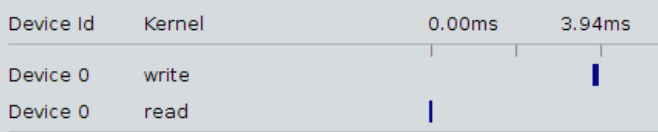
\includegraphics[width=0.7\textwidth]{Figures/profilerow}
\decoRule
\caption[profilerow]{ Dynamic Profiling result for row-stationary Implementation}
\label{fig:rowstatp}
\end{figure}

\begin{table}[]
\centering
\begin{tabular}{|l|c|c|}
\hline
\textbf{Implementation}        & \multicolumn{1}{l|}{\textbf{Execution Time (ms)}} & \multicolumn{1}{l|}{Frequency (MHz)} \\ \hline
\textit{Simple Implementation} & 0.15                                              & 256.1                                \\ \hline
\textit{Sliding Buffer}        & 0.09                                              & 252.8                                \\ \hline
\textit{Row Stationary}        & 3.94                                              & 184.4                                \\ \hline
\end{tabular}
\caption{Results of Part I Test}
\label{tab:resultpartone}
\end{table}

The profiling results and operating frequency of the board for each of the implementations is shown in table \ref{tab:resultpartone}. In the case of the row-stationary implementation, the compute array of processing elements are \emph{autorun} kernels. Therefore they are considered to be running the whole time during execution and will not be caught by the Intel Dynamic Profiler. To approximate the time consumed we take the time difference between the reader and writer kernels that communicate with the grid as the execution time.
Unsurprisingly, the row-stationary implementation is the slowest in a small example. One reason is a low operating frequency due to a long critical path of execution. Another reason is the synchronization and communication overhead between the processing elements in the processing grid. We see also that the sliding buffer has the best performance in the case of a single large image which also makes sense. In the next section we abandon the row-stationary implementation and test the two other kernels in a real-case scenario.


\subsection{Part II : Performance in a Real-Case} 

In \ref{testone} we used a very simple two dimensional convolution to benchmark three different convolution operators. Our row-stationary implementation doesn't support a real-case convolution with multiple input and output channels. For that we compare the two other implementations ( sliding buffer, and optimized implementation \ref{slidingimpl}) configured for a large batch of size of $ 2048 $ and for a convolution requiring multiple input and output channels. This allows us to better compare both operators and to choose which one is more suitable for the LeNet model.

\begin{table}[]
\centering
\begin{tabular}{|l|l|}
\hline
\textbf{Parameter} & \textbf{Value} \\ \hline
Image              & 100x20          \\ \hline
Filter             & 5x5            \\ \hline
Input Channels     & 2             \\ \hline
Output Channels    & 6             \\ \hline
Batch Size         & 2048           \\ \hline
\end{tabular}
\caption{Configuration for Part II Test}
\label{tab:l3params}
\end{table}

The results are shown in table \ref{tab:resultp2}. The sliding buffer is faster in practice, however it comes at the expense of more resources. The difference comes at the expense of a lpwer operating frequency and much higher resource requirements. This may be feasible if we only implement the convolution operation, however in the context of a neural network, we chose the first implementation as we wish to fit more network layers in the same binary. The compiled version of the simple implementation differs from that in reference section as we have removed unrolling factors to lower the resource utilization even more. We have found that kernels with resource utilization >50\% take more than 12 hours to compile and we were unable to run the full compilations without timeouts, memory limits exceeded, and placement errors. The results are fully pipelined for the batch and conform to the theoretical estimate for performance. As compute time for the convolution diminished the effect of buffering kernel coefficients, we estimate the performance taking into consideration only the main computation loop. For the simple implementation the calculation is as follows : \newline Number of cycles = batch size * input ch * output ch * img height * img width * filter height * 
filter width  = $2048 * 2 * 6 * 100 * 20 * 5 * 5 $ = 1,228,800,000 cycles. The frequency of operation is $232.7$ MHz, so we can estimate the time to be 5.28 seconds.
\begin{equation}
 Total Time = \frac{Number of cycles}{Frequency} = \frac{1,288,800,000}{232,700,000}  \approx 5.28 sec
\end{equation}
This result matches to the experimental results. The same calculation can be performed to the case of the sliding buffer implementation. We note that unrolling factors in the sliding buffer reduce the number of cycles, however this is matched by a lower operating frequency as well.

\begin{table}[]
\begin{tabular}{|l|l|l|l|l|}
\hline
\textbf{Implementation}     & \textbf{Total Time (s)} & \textbf{Frequency (MHz)} & \textbf{RAMS} & \textbf{DSP} \\ \hline
\textit{Simple Convolution} & 5.37                    & 232.7                    & 85            & 4            \\ \hline
\textit{Sliding Buffer}     & 3.53                    & 65.1                     & 116           & 51           \\ \hline
\end{tabular}
\label{tab:resultp2}
\caption{Simulation Results of Different Convolution Implementations }
\end{table}


%----------------------------------------------------------------------------------------
\section{Pipelined vs. Non-Pipelined Inference}

In this example we study the effect of pipelining on the inference phase of the neural network. We test both a pipelined implementation of LeNet refernce(section) where kernels are connected by Intel OpenCL Channels and the kernels follow a sliding buffer / streamlined implementation. We also test a non-pipelined version discussed in ref(section),where the operators are run sequentially, communicate through global memory, and exhibit different types of parallelism. The batch size is configurable at runtime, so we test the time it takes for the inference of a single image and the time for a batch of 2048 images. 

The results are that the pipelined version is effectively faster than the non-pipelined version during inference. The figure ref(figure) shows the dynamic profiler results. We note that the kernels were enqueued into separate queues and also in reverse order in the host program. This is why it seems that the softmax kernel has been running the longest, but effectively it only runs after all of the layers have been completed. We noticed that running the kernels in the order that they are supposed to execute introduced latencies due to context switching and the overhead of enqueuing the tasks from the host-side, so this reverse order gives a more accurate representation of time taken. The kernels communicate through channels so we are sure that they are synchronized and the results are verified for correctness by using a LeNet CPU implementation configured with the same weights. The kernel also \emph{effectively} starts running after the reader kernel starts (which is at 0.3ms from the initial start time because it is the last to be launched and all other layers depend on its input). 
The estimation is further verified by running the pipeline to classify a set of 2048 images and the total time taken in that case is 6.12 seconds. A simple calculation in \ref{eqn:check} shows that the theoretical results agree with the experimental results. The dynamic profiler result in \ref{fig:pipebatch} shows that all layers are being effectively utilized in case of batch image inference. 
\begin{equation}
\text{Total time = time for single image * batch size} = 0.03 * 2048 \approx 6.14\text{ seconds}
\label{eqn:check}
\end{equation}

As for the non-pipelined version, we see in \ref{fig:nonpipesingle} that in the case of inference for a single image,  the total time taken for inference is 21.53 milliseconds. Moreover, the effective time by summing up the individual kernel execution times is much less. The reason for the delay in launching kernels is mainly synchronization constructs by calling \emph{clFinish(queue)} in between kernel launches. Summing up individual kernel times leads to an effective execution time of 5.4 milliseconds. This is still lower than the pipelined implementation. For inference of the batch, the effect of synchronization is minimized and we find that the total time of 11.15 seconds meets the theoretical results \ref{eqn:effect}.
 
\begin{equation}
\begin{array}{l}

\text{Batch Execution time = batch size * effective time one image} \\
  \text{        } = 2048 * 0.054 sec \approx 11.05 sec
\end{array}
\label{eqn:effect}
\end{equation}


\begin{table}[]
\begin{tabular}{|l|l|l|}
\hline
Implementation               & \textbf{Single Image (Effective)} & \textbf{Batch of 2048 Images} \\ \hline
\textit{Pipelined LeNet}     & 0.0033 ( 0.003 )                 & 6.12                          \\ \hline
\textit{Non-Pipelined Lenet} & 0.021 ( 0.0054 )                  & 11.15                         \\ \hline
\end{tabular}
\caption{Inference time for pipelined and non-pipelined implementations of Lenet ( in seconds ) }
\label{tab:resultinf}
\end{table}

\begin{figure}[h!]
\centering
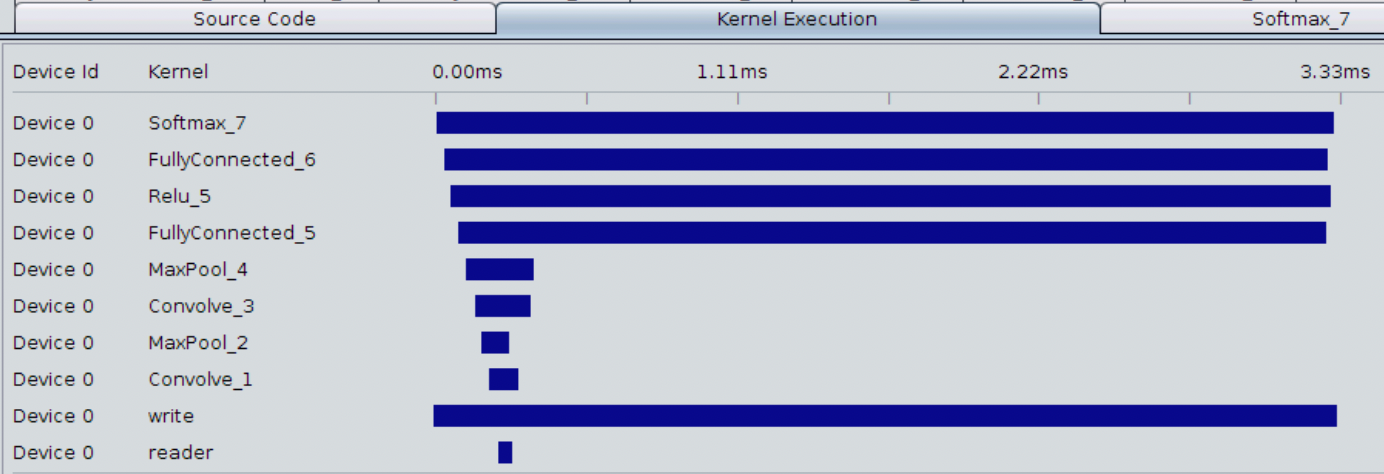
\includegraphics[width=0.85\textwidth]{Figures/pipesingle}
\decoRule
\caption[pipesingle]{ Execution time for inference of a single image (pipelined)}
\label{fig:pipesingle}
\end{figure}

\begin{figure}[h!]
\centering
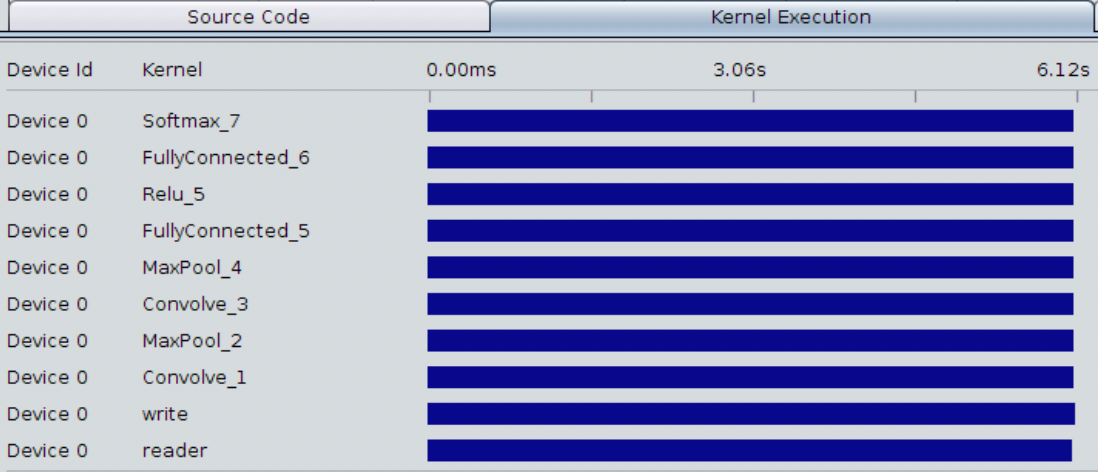
\includegraphics[width=0.85\textwidth]{Figures/pipebatch}
\decoRule
\caption[pipebatch]{ Execution time for inference of a batch of images (pipelined)}
\label{fig:pipebatch}
\end{figure}

\begin{figure}[h!]
\centering
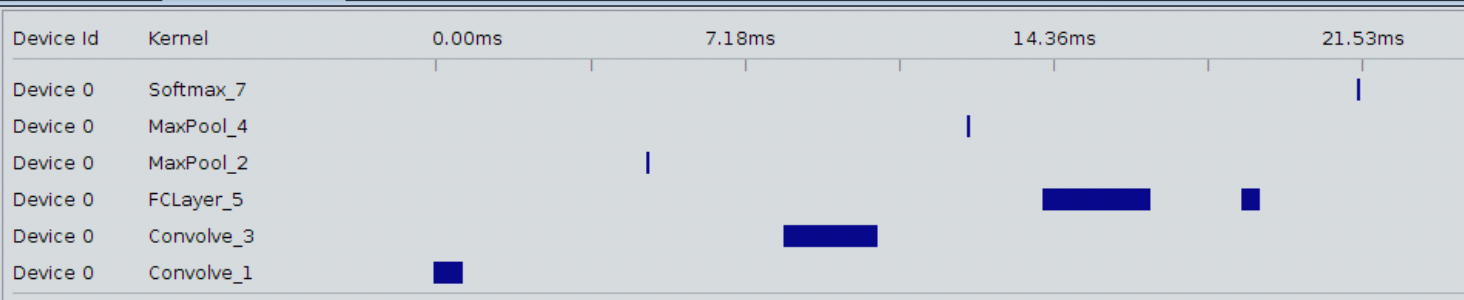
\includegraphics[width=0.85\textwidth]{Figures/nonpipesingle}
\decoRule
\caption[nonpipesingle]{ Execution time for inference of a single image (non-pipelined)}
\label{fig:nonpipesingle}
\end{figure}

\begin{figure}[h!]
\centering
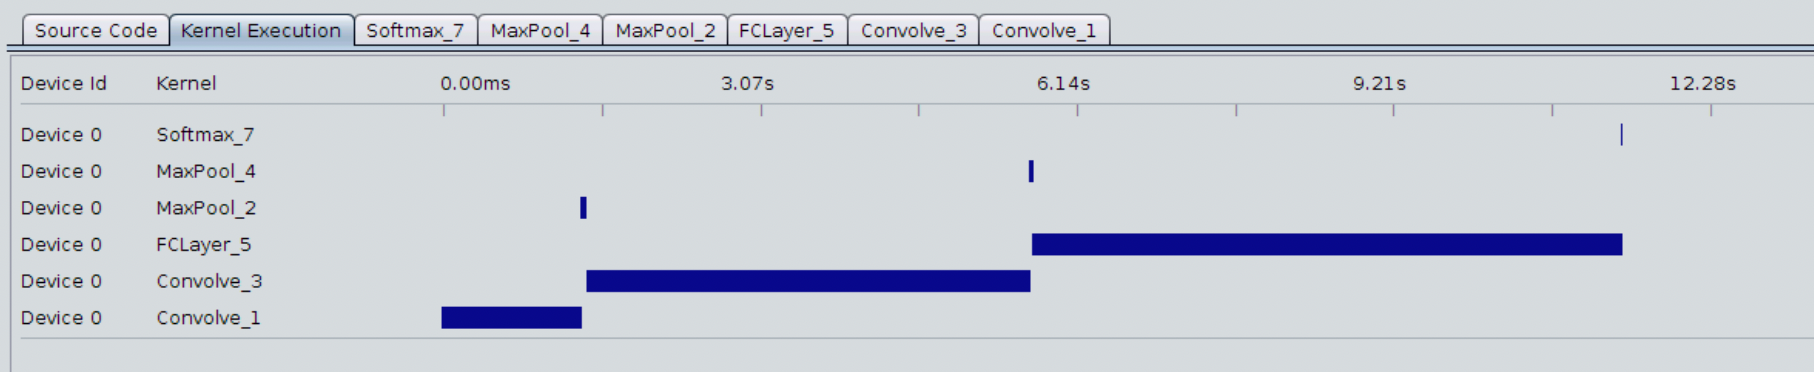
\includegraphics[width=0.85\textwidth]{Figures/nonpipebatch}
\decoRule
\caption[nonpipebatch]{ Execution time for inference of a batch of images (non-pipelined)}
\label{fig:nonpipebatch}
\end{figure}

%----------------------------------------------------------------------------------------

\newpage
\section{Training LeNet}

<needs some coding, then run it > 

%----------------------------------------------------------------------------------------
